%%%%%%%%%%%%%%%%%%%%%%%%%%%%%%%%%%%%%%%%%%%%%%%%%%%%%%%%%%%%%%%%%%%%%%%%%
% sample poster file 
%%%%%%%%%%%%%%%%%%%%%%%%%%%%%%%%%%%%%%%%%%%%%%%%%%%%%%%%%%%%%%%%%%%%%%%%%

%%%%%%%%%%%%%%%%%%%%%%%%%%%%%%%%%%%%%%%%%%%%%%%%%%%%%%%%%%%%%%%%%%%%%%%%%
%% IGL Template
% Last modified: Tue 19 Feb 2013 02:42:39 PM CST
%%%%%%%%%%%%%%%%%%%%%%%%%%%%%%%%%%%%%%%%%%%%%%%%%%%%%%%%%%%%%%%%%%%%%%%%%


%%%%%%%%%%%%%%%%%%%%%%%%%%%%%%%%%%%%%%%%%%%%%%%%%%%%%%%%%%%%%%%%%%%%%%%%%
% documentclass option: pick one:
% "presentation" for powerpoint-like talk,
% "handout" for  printing,
% "trans" for printing onto transparencies
%%%%%%%%%%%%%%%%%%%%%%%%%%%%%%%%%%%%%%%%%%%%%%%%%%%%%%%%%%%%%%%%%%%%%%%%%


%\documentclass[leqno,presentation]{beamer}
\documentclass[leqno, handout]{beamer}
%\documentclass[leqno,trans]{beamer}


%%%%%%%%%%%%%%%%%%%%%%%%%%%%%%%%%%%%%%%%%%%%%%%%%%%%%%%%%%%%%%%%%%%%%%%%%
% beamerposter stuff
%%%%%%%%%%%%%%%%%%%%%%%%%%%%%%%%%%%%%%%%%%%%%%%%%%%%%%%%%%%%%%%%%%%%%%%%%
\usepackage[orientation=landscape, size=a0, scale=1.3]{beamerposter}
\usepackage{pgf}
\usepackage{tikz}
% these packages may be needed 
\usepackage{calc}
\usepackage{times}
\usepackage{type1cm}
\usepackage[latin1]{inputenc}

%%%%%%%%%%%%%%%%%%%%%%%%%%%%%%%%%%%%%%%%%%%%%%%%%%%%%%%%%%%%%%%%%%%%%%%%%
% end beamerposter stuff
%%%%%%%%%%%%%%%%%%%%%%%%%%%%%%%%%%%%%%%%%%%%%%%%%%%%%%%%%%%%%%%%%%%%%%%%%


% load standard packages

\usepackage{amsmath,amssymb, latexsym}
\usepackage[english]{babel}


%\usepackage{hyperref}
%\hypersetup{pdfborderstyle={/S/U/W },pdfborder=0 0 1}

%\usepackage{graphicx}
%\DeclareGraphicsExtensions{.eps, .pdf,.jpg,.png, .tif}

%%%%%%%%%%%%%%%%%%%%%%%%%%%%%%%%%%%%%%%%%%%%%%%%%%%%%%%%%%%%%%%%%%%%%%%%%
% theme
%%%%%%%%%%%%%%%%%%%%%%%%%%%%%%%%%%%%%%%%%%%%%%%%%%%%%%%%%%%%%%%%%%%%%%%%%


%% this seems to work fine

\usetheme{Darmstadt}

%\usetheme{Singapore}


%% beamerposter example uses Berlin, but couldn't get rid of footers 

%\usetheme{Berlin}
%\usetheme{Warsaw}


%\usetheme{PaloAlto}
%\usetheme{AnnArbor}
%\usetheme{CambridgeUS}
%\usetheme{CambridgeUS}
%\usetheme{Berkeley}
%\usetheme{Madrid}


%%%%%%%%%%%%%%%%%%%%%%%%%%%%%%%%%%%%%%%%%%%%%%%%%%%%%%%%%%%%%%%%%%%%%%%%%
%%%%%%%%%%%%%%%%%%%%%%%%%%%%%%%%%%%%%%%%%%%%%%%%%%%%%%%%%%%%%%%%%%%%%%%%%
% begin macros
%%%%%%%%%%%%%%%%%%%%%%%%%%%%%%%%%%%%%%%%%%%%%%%%%%%%%%%%%%%%%%%%%%%%%%%%%
%%%%%%%%%%%%%%%%%%%%%%%%%%%%%%%%%%%%%%%%%%%%%%%%%%%%%%%%%%%%%%%%%%%%%%%%%


% theorem declarations

%\newtheorem{question1}{Question 1}
%\newtheorem{question2}{Question 2}

\theoremstyle{definition}
%\newtheorem{brokenstickproblem}{Broken Stick Problem}




%%%%%%%%%%%%%%%%%%%%%%%%%%%%%%%%%%%%%%%%%%%%%%%%%%%%%%%%%%%%%%%%%%%%%%%%%
%%%%%%%%%%%%%%%%%%%%%%%%%%%%%%%%%%%%%%%%%%%%%%%%%%%%%%%%%%%%%%%%%%%%%%%%%
% end macros
%%%%%%%%%%%%%%%%%%%%%%%%%%%%%%%%%%%%%%%%%%%%%%%%%%%%%%%%%%%%%%%%%%%%%%%%%
%%%%%%%%%%%%%%%%%%%%%%%%%%%%%%%%%%%%%%%%%%%%%%%%%%%%%%%%%%%%%%%%%%%%%%%%%

%%%%%%%%%%%%%%%%%%%%%%%%%%%%%%%%%%%%%%%%%%%%%%%%%%%%%%%%%%%%%%%%%%%%%%%%%
% title/author/date
%%%%%%%%%%%%%%%%%%%%%%%%%%%%%%%%%%%%%%%%%%%%%%%%%%%%%%%%%%%%%%%%%%%%%%%%%

%% size up title and author for poster 

\title{
\veryHuge
Mathematics of Gerrymandering}
  \author{
  \LARGE
Weifan Jiang, Namyoung Kim, Alex Robkin, Leo Segovia, Faculty Mentor: Chris Hoffman, Graduate Mentor: Tejas Devanur}
  

%% uiuc and igl logos DON'T CHANGE ANYTHING HERE
\institute{
%\raisebox{-2ex}{\includegraphics[width=5in]{uwletterhead1.png}}
%\hspace{4em}
%\raisebox{-2ex}{\includegraphics[width=1in]{LogoPDF.pdf}}
%\hspace{1em} 
%\raisebox{-2ex}
%{
\includegraphics[width=1in]{logojpg.jpg}}
%\hspace{1em} 

{\Large{ Washington Experimental Mathematics Lab}}
}


\date{\large Undergraduate Research Symposium 2018 }



%% logo, shows up  in top left corner of each frame
%\logo{%
%\includegraphics[width=0.4in]{igl-logo-small.png}
%}


%%%%%%%%%%%%%%%%%%%%%%%%%%%%%%%%%%%%%%%%%%%%%%%%%%%%%%%%%%%%%%%%%%%%%%%%%


\begin{document}
\begin{frame}

%%%%%%%%%%%%%%%%%%%%%%%%%%%%%%%%%%%%%%%%%%%%%%%%%%%%%%%%%%%%%%%%%%%%%%%%%
% title frame 
%%%%%%%%%%%%%%%%%%%%%%%%%%%%%%%%%%%%%%%%%%%%%%%%%%%%%%%%%%%%%%%%%%%%%%%%%

\begin{block}{}
\titlepage
\end{block}

%%%%%%%%%%%%%%%%%%%%%%%%%%%%%%%%%%%%%%%%%%%%%%%%%%%%%%%%%%%%%%%%%%%%%%%%%
% body of poster
%%%%%%%%%%%%%%%%%%%%%%%%%%%%%%%%%%%%%%%%%%%%%%%%%%%%%%%%%%%%%%%%%%%%%%%%%

\begin{columns}[t]

%%%%%%%%%%%%%%%%%%%%%%%%%%%%%%%%%%%%%%%%%%%%%%%%%%%%%%%%%%%%%%%%%%%%%%%%%
% left column
%%%%%%%%%%%%%%%%%%%%%%%%%%%%%%%%%%%%%%%%%%%%%%%%%%%%%%%%%%%%%%%%%%%%%%%%%

\begin{column}[t]{.25\linewidth}

%%%%%%%%%%%%%%%%%%%%%%%%%%%%%%%%%%%%%%
% left block 1
%%%%%%%%%%%%%%%%%%%%%%%%%%%%%%%%%%%%%%
\begin{block}{Motivation}
Gerrymandering refers to the manipulation of congressional district boundaries to favor a particular political party. Our goal is to determine how likely it is that a given state's map is gerrymandered. We began with the state of Iowa. To do this, we approximate and analyze the distribution of all possible redistrictings and determine how similar the current district map is to samples from this distribution.
\\
We consider:
\begin{itemize}
\item How to quantify state and federal laws for congressional redistricting.
\item How to sample from such a large distribution (Iowa alone has $\approx 4^{99}$ potential redistrictings).
\end{itemize}
 
% \begin{itemize}
%  \item Apollonius (2nd century BCE)---discovered that given three mutually tangent circles, exactly two circles are tangent to all three
%  \item Rene Descartes (17th century CE)---related the radii of three mutually tangent circles and a fourth that is outside and tangent to the original three
%  \item Frederick Soddy (1937)---rediscovered Descartes' formula and extended to three-dimensions
% \end{itemize}

\end{block}
%%%%%%%%%%%%%%%%%%%%%%%%%%%%%%%%%%%%%%
% end left block 1
%%%%%%%%%%%%%%%%%%%%%%%%%%%%%%%%%%%%%%

%%%%%%%%%%%%%%%%%%%%%%%%%%%%%%%%%%%%%%
% left block 2
%%%%%%%%%%%%%%%%%%%%%%%%%%%%%%%%%%%%%%
\begin{block}{Redistricting Requirements and Energies}
 
We use the The Metropolis Hastings (M.H.) algorithm to produce a random walk that has as its unique stationary distribution, the ideal probability distribution $p$, of all possible districting plans for a given U.S state.

\medskip

For Iowa, our model incorporates the redistricting requirements as "energies", measuring the compactness of districts and their population variation. The total energy is a linear combination of these energies.

\medskip

Population energy:
\[\sum_{Districts}\left(\text{District Pop.}- \frac{\text{State pop.}}{\text{Number of districts}}\right)^2\]

\medskip

Compactness energy:
\[\sum_{Districts}\frac{\text{(District perimeter)}^2}{\text{District area}}\]

We begin the random walk with an arbitrary sample from our distribution. We then choose a similar sample randomly and accept with a certain probability. If we choose not to accept, we stay at the current sample. This  process repeats for several iterations. 

\medskip

Accept candidate with probability:
\[\text{min}\left(1,\frac{\textnormal{exp(weighted sum of current energies})}{\textnormal{exp(weighted sum of candidate energies})}\right)\]

\end{block}
%%%%%%%%%%%%%%%%%%%%%%%%%%%%%%%%%%%%%%
% end left block 2
%%%%%%%%%%%%%%%%%%%%%%%%%%%%%%%%%%%%%%

%%%%%%%%%%%%%%%%%%%%%%%%%%%%%%%%%%%%%%
% left block 3
%%%%%%%%%%%%%%%%%%%%%%%%%%%%%%%%%%%%%%

%%%%%%%%%%%%%%%%%%%%%%%%%%%%%%%%%%%%%%
% end left block 3
%%%%%%%%%%%%%%%%%%%%%%%%%%%%%%%%%%%%%%


\end{column}

%%%%%%%%%%%%%%%%%%%%%%%%%%%%%%%%%%%%%%%%%%%%%%%%%%%%%%%%%%%%%%%%%%%%%%%%%
% end left column
%%%%%%%%%%%%%%%%%%%%%%%%%%%%%%%%%%%%%%%%%%%%%%%%%%%%%%%%%%%%%%%%%%%%%%%%%


%%%%%%%%%%%%%%%%%%%%%%%%%%%%%%%%%%%%%%%%%%%%%%%%%%%%%%%%%%%%%%%%%%%%%%%%%
% middle column, wide
%%%%%%%%%%%%%%%%%%%%%%%%%%%%%%%%%%%%%%%%%%%%%%%%%%%%%%%%%%%%%%%%%%%%%%%%%

\begin{column}{.45\linewidth}

%%%%%%%%%%%%%%%%%%%%%%%%%%%%%%%%%%%%%%
% center block 1
%%%%%%%%%%%%%%%%%%%%%%%%%%%%%%%%%%%%%%
%\begin{block}
%\end{block}
\begin{columns}[t]
\begin{column}{.48\linewidth}
\begin{block}{Simulation Statistics}
\vspace{1ex}
\begin{figure}
		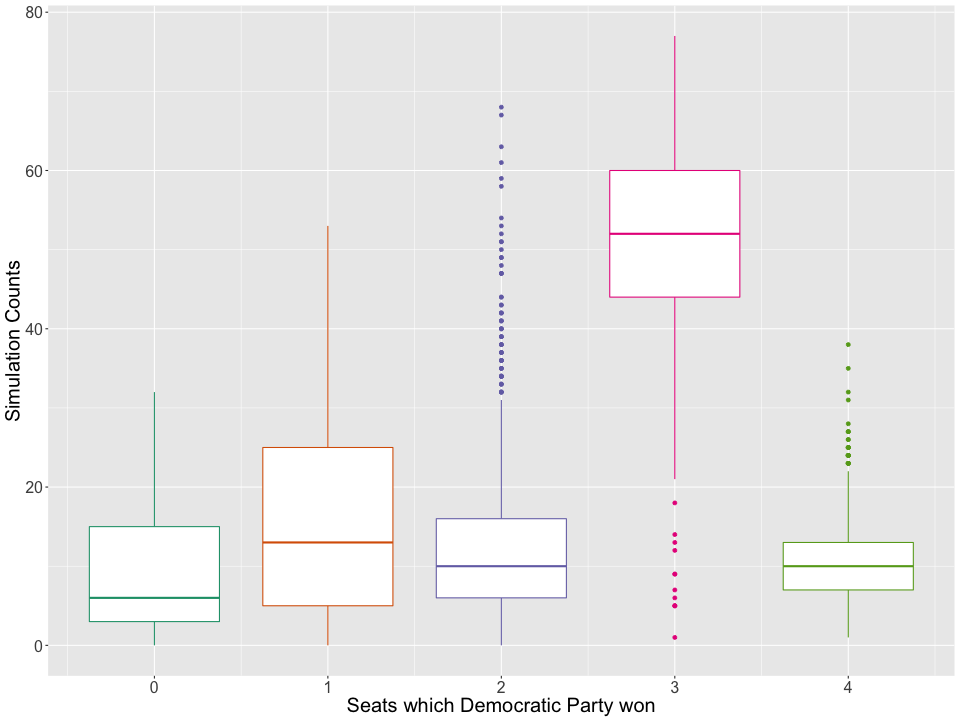
\includegraphics[width=25cm]{boxplot.png}\\
		\caption{Box plot of 100 election samples for 1000 redistricted maps each. For seats 0, 1, 2, 3, 4, averages are 9.105, 15.867, 12.726, 51.493, 10.809 respectively and standard deviations are 7.57954, 12.34146, 10.216, 11.71167, 4.94459.}
		\end{figure}

%\begin{figure}
%		\includegraphics[width=25cm]{hhh.jpg}\\
		%\caption{}
		%\end{figure}


\end{block}
\begin{block}{Actual Iowa District Map with Election Simulation}

\begin{figure}
		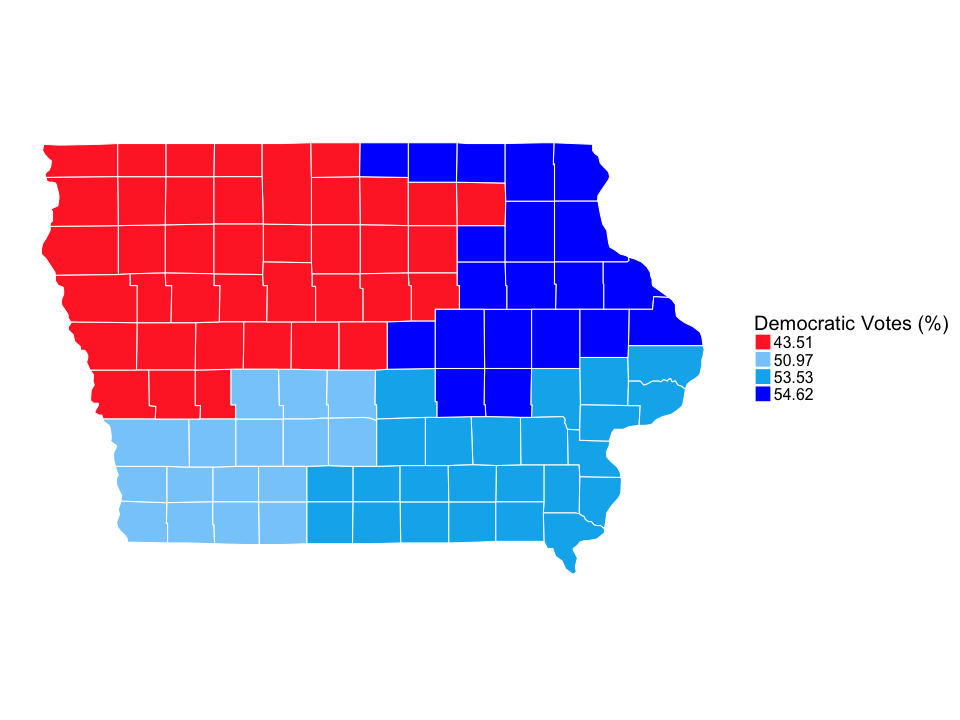
\includegraphics[width=25cm]{actual.png}\\
		\caption{Iowa's Congressional districts since 2013. For 1000 election simulation, Democratic party got 0 seat 194 times, 1 seat 43 times, 2 seats 99, 3 seats 475, 4 seats 189. This map is one example of 3 seats case.}
		\end{figure}

\end{block}
\end{column}


\begin{column}[t]{.48\linewidth}
\begin{block}{Redistricted Maps and Election Simulation}
\vspace{1ex}
\begin{figure}
		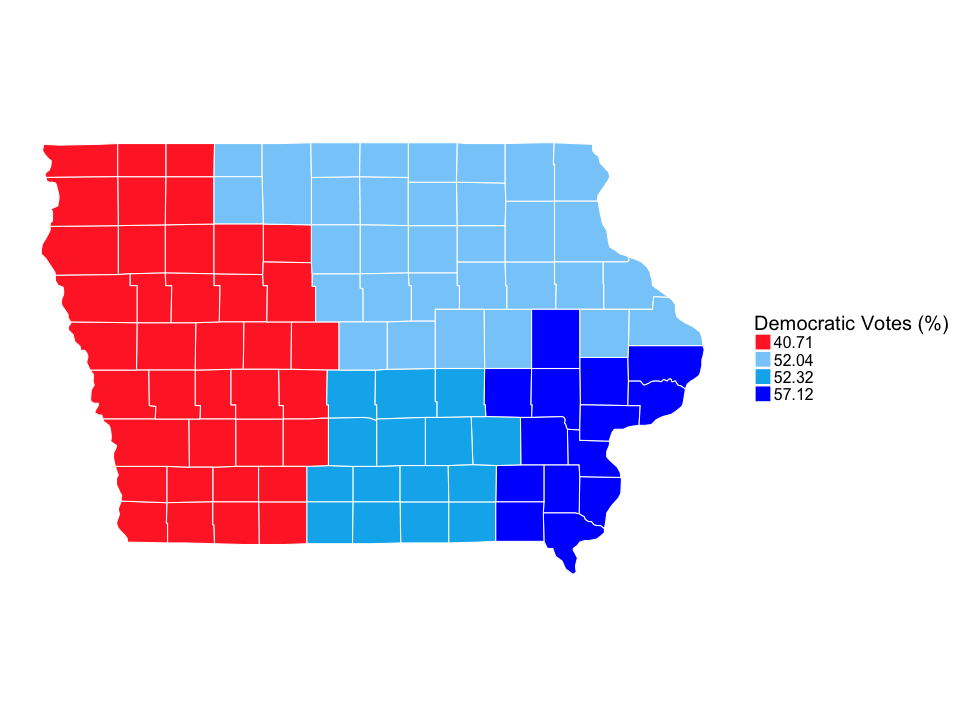
\includegraphics[width=25cm]{redistricting990.png}\\
		\caption{For 1000 election simulation, Democratic party got 0 seat 54 times, 1 seat 171 times, 2 seats 138, 3 seats 550, 4 seats 87. This map is one example of 3 seats case. }
		\end{figure}

\begin{figure}
		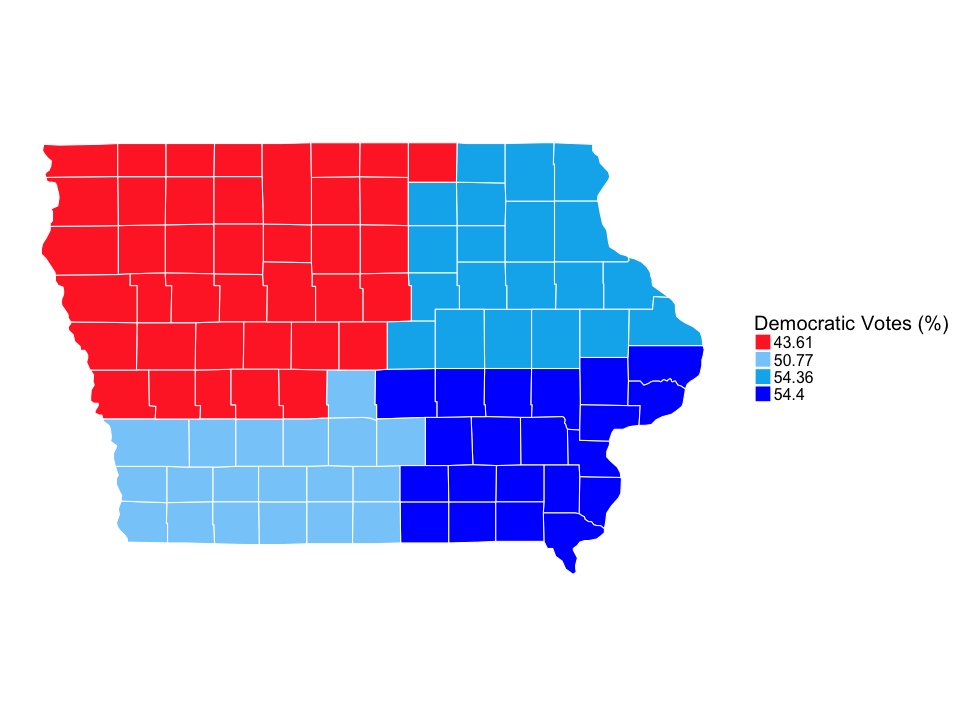
\includegraphics[width=25cm]{redistricting1000.png}\\
		\caption{For 1000 election simulation, Democratic party got 0 seat 231 times, 1 seat 28 times, 2 seats 161, 3 seats 432, 4 seats 148. This map is one example of 3 seats case. }
		\end{figure}


\end{block}
\end{column}
\end{columns}
%\end{block}
%%%%%%%%%%%%%%%%%%%%%%%%%%%%%%%%%%%%%%
% end center block 1
%%%%%%%%%%%%%%%%%%%%%%%%%%%%%%%%%%%%%%


\end{column}

%%%%%%%%%%%%%%%%%%%%%%%%%%%%%%%%%%%%%%%%%%%%%%%%%%%%%%%%%%%%%%%%%%%%%%%%%
% end middle column, wide
%%%%%%%%%%%%%%%%%%%%%%%%%%%%%%%%%%%%%%%%%%%%%%%%%%%%%%%%%%%%%%%%%%%%%%%%%


%%%%%%%%%%%%%%%%%%%%%%%%%%%%%%%%%%%%%%%%%%%%%%%%%%%%%%%%%%%%%%%%%%%%%%%%%
% right column, narrow 
%%%%%%%%%%%%%%%%%%%%%%%%%%%%%%%%%%%%%%%%%%%%%%%%%%%%%%%%%%%%%%%%%%%%%%%%%

\begin{column}{.25\linewidth}

%%%%%%%%%%%%%%%%%%%%%%%%%%%%%%%%%%%%%%
% right block 1
%%%%%%%%%%%%%%%%%%%%%%%%%%%%%%%%%%%%%%
%\begin{block}{Redistricting Requirements and Energies}

%\

%\end{block}
%%%%%%%%%%%%%%%%%%%%%%%%%%%%%%%%%%%%%%
% end right block 1
%%%%%%%%%%%%%%%%%%%%%%%%%%%%%%%%%%%%%%

%%%%%%%%%%%%%%%%%%%%%%%%%%%%%%%%%%%%%%
% right block 1.5
%%%%%%%%%%%%%%%%%%%%%%%%%%%%%%%%%%%%%%
\begin{block}{Evaluation of samples and Optimization}
After we generated samples of redistricting plans, we wanted to make sure that we sampled correctly. Which means that:
	\begin{itemize}
    \item The final shape of districts must stay reasonably-compact (no S-shaped, no strips)
    \item The sum of the difference between each district's actual population and average district population must be within $4\%$ of Iowa's total population
	\end{itemize}
We want the samples to be independent from the initial map. We consider the following events as indicators of independence:
%We have found some trends in the final samples as events:
	\begin{itemize}
    \item Whether two counties belong to the same district (we considered Story county and Tama county).
    \item Whether there is a land-locked district (not touching state boundaries)
	\end{itemize}
The independence tests are quantified by calculating "if such event happens in initial map, is it likely to happen in the final sample?"

We decided to use simulated-annealing to preserve both independence and quality. The first half of the random walk has low weights of energies to move away from the initial sample. During the second half, parameters increase to move towards samples with increasing quality.
\end{block}
%%%%%%%%%%%%%%%%%%%%%%%%%%%%%%%%%%%%%%
% end right block 1.5
%%%%%%%%%%%%%%%%%%%%%%%%%%%%%%%%%%%%%%

%%%%%%%%%%%%%%%%%%%%%%%%%%%%%%%%%%%%%%
% right block 2
%%%%%%%%%%%%%%%%%%%%%%%%%%%%%%%%%%%%%%
% \begin{block}{Future Work}
%We will define a majority-minority energy equation in a way that ensures minority populations have an equal opportunity to elect representatives of their choice. We will also define a counties-split energy equation such that the division cities and counties should be minimized. 

%This study will help to determine if the current redrawn maps legitimately reflect the people they purport to represent. The next state we will be applying our model to will be the state of Washington.
%\end{block}
%%%%%%%%%%%%%%%%%%%%%%%%%%%%%%%%%%%%%%
% end right block 2
%%%%%%%%%%%%%%%%%%%%%%%%%%%%%%%%%%%%%%

\begin{block}{Election Simulation}
We generated a multivariate normal distribution based on the past three presidential election results for Iowa counties. We used these results to simulate congressional elections on 1000 maps generated by the M.H, algorithm, recording the average number of seats won by Democrats in these elections. 
\end{block}

%%%%%%%%%%%%%%%%%%%%%%%%%%%%%%%%%%%%%%
% right block 3
%%%%%%%%%%%%%%%%%%%%%%%%%%%%%%%%%%%%%%
\begin{block}{References}
Bangia, S., Dou, B., Guo, S., Mattingly, J., \& Vaughn, C. (n.d.). Quantifying Gerrymandering.
% \begin{itemize}
% \item Athreya, J., Boca, F., and Zaharescu, A. ``Radial density in Apollonian circle packings.'' In preparation.

% \item Kontorovich, A. ``The Local-Global Principle for Integral Soddy Sphere Packings.'' arXiv:1208.5441.

% \item Marden, A. \emph{Outer circles: an introduction to hyperbolic 3-manifolds.} Cambridge: Cambridge University Press, 2007.
% \end{itemize}
\end{block}
%%%%%%%%%%%%%%%%%%%%%%%%%%%%%%%%%%%%%%
% end right block 3
%%%%%%%%%%%%%%%%%%%%%%%%%%%%%%%%%%%%%%

\end{column}
%%%%%%%%%%%%%%%%%%%%%%%%%%%%%%%%%%%%%%%%%%%%%%%%%%%%%%%%%%%%%%%%%%%%%%%%%
% end right column
%%%%%%%%%%%%%%%%%%%%%%%%%%%%%%%%%%%%%%%%%%%%%%%%%%%%%%%%%%%%%%%%%%%%%%%%%

\end{columns}
%%%%%%%%%%%%%%%
%Funding Acknowledgements: Make sure you get this right before sending to printers
%%%%%%%%%%%%%%%

\vfill

  \begin{block}{}
   \begin{center}
This poster is made with support from the Washington Expiremental Mathematics Lab at the University of Washington at Seattle.
  \end{center}
  \end{block}



\end{frame}
\end{document}